% Figure 4: Merkle-Tree Provenance Certificate
\documentclass[tikz,border=5pt]{standalone}
\usepackage{tikz}
\usetikzlibrary{arrows.meta,positioning,calc}

\begin{document}
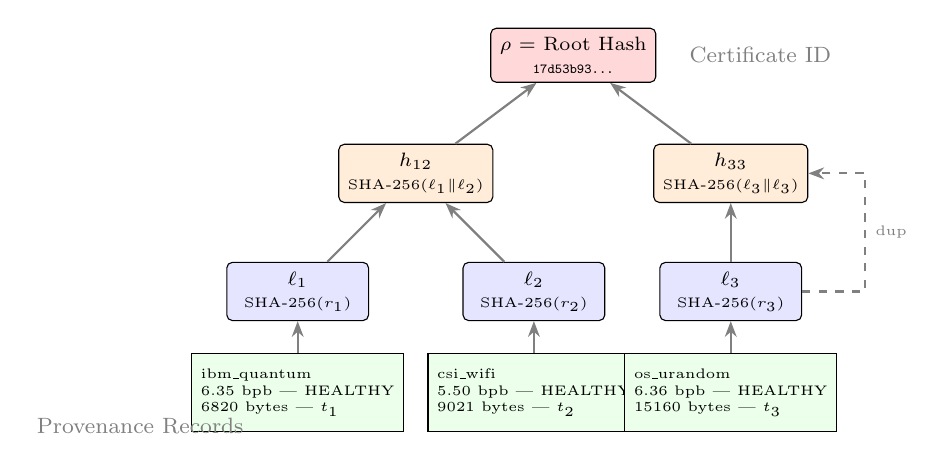
\begin{tikzpicture}[
  node/.style={draw, rounded corners=2pt, minimum width=1.8cm, minimum height=0.6cm, align=center, font=\scriptsize},
  root/.style={node, fill=red!15},
  inner/.style={node, fill=orange!15},
  leaf/.style={node, fill=blue!10},
  arr/.style={-{Stealth[length=2mm]}, thick, gray},
]

% Root
\node[root] (root) at (4, 4.5) {$\rho$ = Root Hash\\{\tiny\texttt{17d53b93...}}};

% Level 1
\node[inner] (h12) at (2, 3) {$h_{12}$\\{\tiny SHA-256($\ell_1 \| \ell_2$)}};
\node[inner] (h33) at (6, 3) {$h_{33}$\\{\tiny SHA-256($\ell_3 \| \ell_3$)}};

% Leaves
\node[leaf] (l1) at (0.5, 1.5) {$\ell_1$\\{\tiny SHA-256($r_1$)}};
\node[leaf] (l2) at (3.5, 1.5) {$\ell_2$\\{\tiny SHA-256($r_2$)}};
\node[leaf] (l3) at (6, 1.5) {$\ell_3$\\{\tiny SHA-256($r_3$)}};

% Records
\node[draw, fill=green!8, minimum width=2.5cm, minimum height=1cm, align=left, font=\tiny, below=0.4cm of l1] (r1) {
  ibm\_quantum\\
  6.35 bpb | HEALTHY\\
  6820 bytes | $t_1$
};
\node[draw, fill=green!8, minimum width=2.5cm, minimum height=1cm, align=left, font=\tiny, below=0.4cm of l2] (r2) {
  csi\_wifi\\
  5.50 bpb | HEALTHY\\
  9021 bytes | $t_2$
};
\node[draw, fill=green!8, minimum width=2.5cm, minimum height=1cm, align=left, font=\tiny, below=0.4cm of l3] (r3) {
  os\_urandom\\
  6.36 bpb | HEALTHY\\
  15160 bytes | $t_3$
};

% Arrows
\draw[arr] (h12) -- (root);
\draw[arr] (h33) -- (root);
\draw[arr] (l1) -- (h12);
\draw[arr] (l2) -- (h12);
\draw[arr] (l3) -- (h33);
\draw[arr, dashed] (l3.east) -- ++(0.8,0) |- (h33.east) node[pos=0.25, right, font=\tiny, text=gray] {dup};
\draw[arr] (r1) -- (l1);
\draw[arr] (r2) -- (l2);
\draw[arr] (r3) -- (l3);

% Labels
\node[font=\footnotesize, gray, right=0.3cm of root] {Certificate ID};
\node[font=\footnotesize, gray] at (-1.5, -0.2) {Provenance Records};

\end{tikzpicture}
\end{document}
